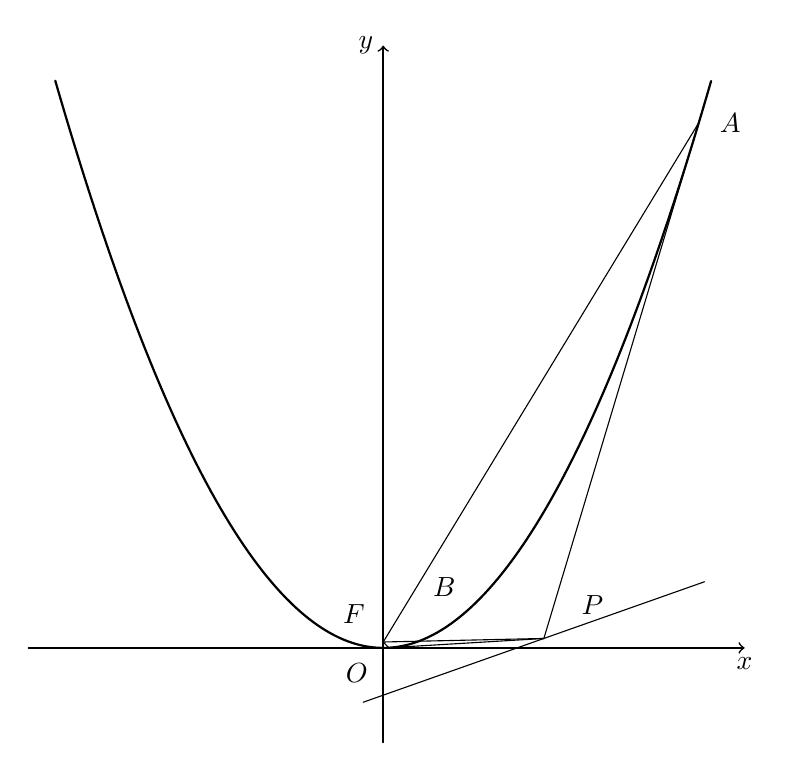
\begin{tikzpicture}[line width=.6pt,line join=round,line cap=round,x=0.85cm,y=0.3cm]
\draw[->] (-5.3,0) -- (5.4,0) node[below] {$x$};
\draw[->] (0,-4) -- (0,25.5) node[left] {$y$};
\node[below left=2pt] at (0,0) {$O$};
\draw[line width=.8pt] plot[domain=-4.9:4.9,samples=140] (\x,{\x*\x});
\draw[thin] (-0.3,-2.3) -- (4.8,2.8);
\coordinate (P) at (2.4000000000,0.4000000000);
\coordinate (A) at (4.7151673806,22.2328034267);
\coordinate (B) at (0.0848326194,0.0071965733);
\coordinate (F) at (0,0.25);
\draw[thin] (P)--(A);
\draw[thin] (P) -- (B);
\draw[thin] (F) -- (A);
\draw[thin] (F) -- (P);
\draw[thin] (F) -- (B);


\node[right=4pt] at (A) {$A$};
\node[right=10pt,yshift=12pt] at (P) {$P$};
\node[above=5pt,xshift=20pt,yshift=10pt] at (B) {$B$};
\node[above left=3pt] at (F) {$F$};
\end{tikzpicture}
